\documentclass[preprint,12pt]{elsarticle}

\usepackage[brazil]{babel}
\usepackage[utf8]{inputenc}

\usepackage[a4paper,top=3cm,bottom=2cm,left=3cm,right=3cm,marginparwidth=1.75cm]{geometry}

%% Useful packages
\usepackage{amsmath}
\usepackage{graphicx}
\usepackage{subcaption}
\usepackage{booktabs}
\usepackage{xcolor}
\usepackage{listings}
\usepackage{textcomp}
\usepackage{float}
\usepackage{caption}
\usepackage{lineno}
\usepackage{amssymb}
\usepackage{graphicx}
\usepackage{array}
\usepackage{mathtools}
\usepackage[numbers]{natbib}


\usepackage[colorinlistoftodos]{todonotes}
\usepackage[colorlinks=true, allcolors=blue]{hyperref}
\captionsetup{compatibility=false}
\usepackage{url}
\usepackage{multirow}
\usepackage{makecell}

\usepackage{etoolbox}
\patchcmd{\abstract}{Abstract}{Resumo}{}{}

%% Removing lines when no abstract is given
\makeatletter
\renewcommand{\MaketitleBox}{
	\resetTitleCounters
	\def\baselinestretch{1}
	\begin{center}
		\def\baselinestretch{1}
		\Large \@title \par
		\vskip 18pt
		\normalsize\elsauthors \par
		\vskip 10pt
		\footnotesize \itshape \elsaddress \par
	\end{center}
	\vskip 12pt
}
\makeatother

%% Removing custom footer on first page
\makeatletter
\def\ps@pprintTitle{
	\let\@oddhead\@empty
	\let\@evenhead\@empty
	\def\@oddfoot{\centerline{\thepage}}
	\let\@evenfoot\@oddfoot
}
\makeatother

\newcommand{\red}[1]{\textcolor{red}{#1}}
\newcommand{\blu}[1]{\textcolor{blue}{#1}}
\newcommand{\score}[2]{\blu{#1}$\times$\red{#2}}

\begin{document}
		
\title{Construção de modelos baseados em agentes utilizando técnicas de inteligência artificial para jogos de computadores}
\author{Victor Teixeira de Melo Mayrink}
\address{MAC5784 - Inteligência Artificial em Jogos de Computador}

\begin{abstract}
	Este trabalho apresenta uma metodologia para construir modelos baseados em agentes, em combinação com algumas técnicas de inteligência artificial que normalmente são utilizadas no contexto de jogos de computador. A metodologia proposta é ilustrada através da implementação de dois modelos distintos: o primeiro simula o fluxo de pessoas atravessando uma estação de metrô em sentidos opostos; o segundo modelo simula um jogo clássico em que dois times adversários competem para capturar a bandeira do oponente. Os aspectos práticos de implementação são discutidos em detalhes, assim como os resultados observados e as conclusões realizadas.
\end{abstract}

\maketitle

\section{Introdução}
\label{sec:intro}

A modelagem baseada em agentes é um paradigma para construção de modelos computacionais a partir de entidades autônomas, chamadas \textit{agentes}, capazes de interagir entre si e com o ambiente onde estão inseridas.

Um dos primeiros e mais conhecidos modelos baseados em agentes foi publicado em 1971 por Thomas Schelling, ao demonstrar como grupos étnicos diferentes tendem a se segregar ao longo do tempo. O resultado observado foi surpreendente: se cada indivíduo (ou família) possuir uma preferência em residir próximo de pessoas do mesmo grupo étnico, então os diferentes grupos tendem a se segregar de forma muito expressiva ao longo do tempo, mesmo que a preferência por vizinhos do mesmo grupo seja muito pequena.

Apesar de bastante simples, o modelo de Schelling permitiu extrair conclusões interessantes sobre o comportamento social dos indivíduos e explicar porque é tão difícil combater o problema de segregação. Na prática, ao modelar sistemas a partir dos níveis hierárquicos mais básicos (por exemplo, o comportamento de um indivíduo), em geral é possível observar um certo nível de auto-organização. Muitas vezes, padrões e comportamentos que não foram explicitamente programados emergem através da interação entre os agentes \cite{macal2010tutorial}.

A utilização de modelos baseados em agentes têm ganhado bastante interesse nas dua últimas décadas. As aplicações estendem-se em uma grande diversidade pesquisas; podemos destacar, por exemplo, trabalhos relevantes na área de ecologia \cite{grimm2006standard} e ciências sociais \cite{bonabeau2002agent}. 

O escopo deste trabalho, no entanto, têm como objetivo combinar o paradigma de modelagem baseada em agentes com técnicas de inteligência artificial comumente empregadas no contexto de jogos de computadores.

\newpage

Conforme menciona \citet{millington2016artificial}, a modelagem baseada em agentes no contexto de jogos de computadores está relacionada à criação de personagens que são capazes de: $i)$ capturar informações sobre estado corrente do jogo (sensoreamento); $ii)$ analisar quais ações podem ser tomadas com base nas informações observadas; e $iii)$ executar a ação mais adequada tendo em vista um objetivo a ser alcançado.

Para ilustrar a combinação destas duas técnicas, este trabalho descreve a modelagem de dois problemas diferentes. O primeiro modelo é uma simulação do fluxo de passageiros cruzando uma estação de metrô em sentidos opostos. Este modelo têm como objetivo construir um cenário que seja visualmente realista; sem, contudo, levar em consideração questões técnicas muito detalhadas, como por exemplo: o espaço médio ocupado por uma pessoa, a concentração máxima de pessoas por metro quadrado, ou ainda a função distribuição de probabilidades da velocidade em que as pessoas se movimentam nessas estações. Portanto, esse modelo simplificado da realidade, possivelmente não seria adequado para simular, por exemplo, uma situação de evacuação de uma estação em casos emergência. No entanto, tal modelo certamente seria útil para construir uma animação visualmente realista deste tipo de situação.

O segundo modelo, inserido no contexto dos jogos de computador, simula uma competição entre duas equipes adversárias que disputam para capturar a bandeira do oponente e levá-la até uma região previamente delimitada. Neste contexto, o objetivo é construir uma estratégia suficientemente inteligente para competir com um jogador humano que esteja no comando de uma das equipes. O principal requisito, neste caso, é que o comportamento da equipe que está sendo simulada responda coerentemente às ações que seu adversário executa ao longo da partida.

O presente trabalho foi dividido da seguinte maneira: a próxima seção descreve os objetivos gerais deste estudo. Em seguida, na seção 3, discutimos os principais conceitos do paradigma de modelagem baseada em agentes, incluindo alguns detalhes práticos de implementação. As seções 4 e 5 apresentam os modelos da estação de metrô e do jogo da bandeira, respectivamente. Finalmente, a seção 6 apresenta os resultados observados, e a seção 7 discute as conclusões do trabalho.

\section{Objetivos}
\label{sec:objetivos}

Os objetivos desse trabalho são:

\begin{enumerate}
	\item Discutir os princípios da modelagem baseada em agentes;
	\item Ilustrar a utilização do paradigma de modelagem baseada em agentes no contexto dos jogos de computador;
	\item Demonstrar o processo de modelagem do comportamento individual dos agentes utilizando técnicas de inteligência artificial;
	\item Analisar os comportamentos coletivos que emergem da interação entre vários agentes inseridos em um mesmo ambiente;
	\item Apresentar como é possível extrair conclusões úteis sobre problemas realistas a partir de uma análise da simulação de um modelo computacional relativamente simples.
\end{enumerate}

\newpage

\section{Modelagem baseada em agentes}
\label{sec:agentes}

A modelagem baseada em agentes é um paradigma centrado no comportamento individual dos elementos que fazem parte de um sistema. Esta perspectiva contrasta com os métodos tradicionais de modelagem, como por exemplo simulações numéricas baseadas em equações diferenciais, que descrevem o comportamento de um sistema seguindo uma abordagem holística.

Conforme com \citet{macal2005tutorial}, a construção de um modelo baseado em agentes envolve as seguintes etapas:

\begin{enumerate}
	\item identificar quais agentes do sistema e uma teoria sobre como esses agentes se comportam;
	\item identificar o relacionamento entre os agentes e uma teoria sobre como e quando as interações acontecem;
	\item coletar dados sobre o comportamento real dos agentes e do sistema que está sendo modelado;
	\item validar o comportamento dos agentes e do modelo como um todo, utilizando os dados obtidos;
	\item executar a simulação do modelo e analisar os resultados observados, relacionando os comportamentos em micro e macro escala.
\end{enumerate}

Evidentemente, dependendo do tipo de aplicação, nem todos os requisitos acima são absolutamente necessários para um modelo baseado em agentes. Por exemplo, no contexto de jogos de computadores, as etapas de coleta e validação de dados, apesar de útil, pode não ser necessária;  basta que o modelo atenda o objetivo final do problema, que é construir um cenário fictício em que os personagens atuem de forma coerente com seus objetivos no jogo.

Contudo, se o problema em questão for a simular a evacuação de um shopping center em caso de incêndio; onde o objetivo é projetar e dimensionar as saídas de emergências do prédio, então é muito importante validar a teoria sobre o comportamento das pessoas em situações de pânico, garantir que o modelo criado seja o mais semelhante possível da realidade.

\subsection{Implementação computacional dos modelos}
\label{subsec:implementacao}

O modelo computacional de um agente deve possuir variáveis de estado, como por exemplo sua posição geográfica ou a velocidade que ele se movimenta. Dependendo do tipo de problema, algumas desses atributos podem ser variáveis ou fixos durante a simulação. Muitas vezes é importante garantir que a população de agentes tenha características heterogêneas, por exemplo agentes que se movimentam com velocidades diferentes, ou que tenham comportamentos mais agressivos doo que outros.

Da mesma forma, o ambiente também tem um estado que pode ser influenciado pelas ações do agentes, ou simplesmente pela sua própria presença, conforme discutiremos no caso dos agentes que possuem um mapa de influência no ambiente.

O comportamento dos agentes pode ser implementado por funções que podem alterar o estado de um ou mais agentes, ou do próprio ambiente.

Diante do exposto, do ponto de vista técnico é bastante natural adotar o paradigma de programação orientada à objetos para construir modelos baseados em agentes. Desta forma podemos pensar em cada agente da simulação como sendo uma instância de uma classe, com atributos e métodos próprios. 

Nos modelos baseados em agentes a simulação se passa em instantes discretos de tempo, denominados \textit{ticks}, que correspondem às iterações da simulação. A cada passo de tempo, um ou mais agentes são \textit{ativados}. Ao ser ativado, o agente pode ter a oportunidade de tomar uma ação, o que lhe permite alterar o seu próprio estado e interagir com outro agente e/ou com o ambiente.

No entanto, do ponto de vista computacional, não é possível ativar todos os agentes simultaneamente. Mesmo utilizando técnicas de computação paralela, em geral a quantidade de agentes de um modelo é maior que o número de núcleos de processamento da máquina. Além disso, podem haver partes do código que não são paralelizáveis. A ordem em que os agentes são ativados dentro de um mesmo \textit{tick} é controlada por um componente do modelo chamado \textit{scheduler}. Por exemplo, os agentes podem ser ativados em uma ordem aleatória, ou seguir sempre uma determinada ordem pré-definida.

Finalmente, ainda de acordo com \cite{macal2005tutorial}, podemos resumir o processo de implementação de um modelo baseado em agentes nas seguintes etapas:

\begin{enumerate}
	\item Agentes: identificar os tipos de agentes e outros objetos (classes), juntamente com seus atributos;
	\item Ambiente: definir o ambiente em que os agentes irão viver e interagir;
	\item Métodos dos Agentes: especificar um conjunto de métodos em que o estado dos agentes é atualizado em resposta às interações agente-agente e agente-ambiente;
	\item Interações: especificar os métodos que controlam quais agentes interagem, quando interagem e como interagem;
	\item Implementação: implementar o modelo de agentes em algum software ou linguagem de programação.
\end{enumerate}

Os modelos desenvolvidos neste trabalho foram desenvolvidos na linguagem \textit{python} utilizando a biblioteca \textit{mesa} \cite{mesa2017agent}, que implementa um \textit{framework} para facilitar a criação de modelos baseados em agentes.

\section{Fluxo de passageiros em uma estação de metrô}
\label{sec:metro}

Este experimento simula o fluxo de passageiros em uma estação de metrô. O cenário criado possui apenas dois acessos, e o objetivo dos passageiros é atravessar a estação até a saída localizada no lado oposto. A figura \ref{fig:metro} ilustra esse cenário em um determinado instante da simulação.

\begin{figure}
	\centering
	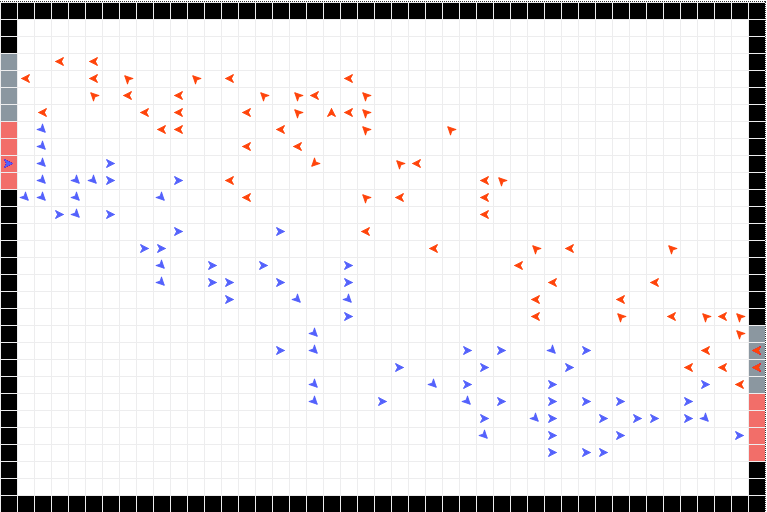
\includegraphics[totalheight=5cm]{figures/metro.png}
	\caption{Simulação do fluxo de pessoas em uma estação de metrô}
	\label{fig:metro}
\end{figure}

Nesta simulação existem 3 tipos diferentes de agentes:

\begin{itemize}
	\setlength\itemsep{0pt}
	\item roletas (\textit{gate}): representam os acessos da estação, sua função é inserir e/ou remover os passageiros no ambiente da simulação.
	\item passageiros (\textit{walker}): são criados continuamente nas roletas e movimentam-se em direção à saída do lado oposto. Ao alcançarem a saída, são removidos da simulação.
	\item barreira (\textit{wall}): é um agente auxiliar, sua única função é obstruir a movimentação dos passageiros.
\end{itemize}

O cenário da estação de metrô foi construído com uma malha (\textit{grid}) de $45 \times 30$ células. Os \textit{passageiros} podem movimentar-se somente sobre as \textit{roletas} e células vazias que estejam dentro da vizinhança de sua posição atual (considerando uma vizinhança de \textit{Moore} com raio unitário). Não é permitido que dois ou mais passageiros ocupem uma mesma célula simultaneamente. 

A cada passo de tempo, os agentes do tipo \textit{roleta} verificam se algum \textit{passageiro} vindo da direção oposta chegou até a sua posição; em caso positivo, este agente é removido da simulação. Em seguida, a \textit{roleta} tem uma probabilidade $\rho$ de criar um novo passageiro que irá seguir em direção à saída oposta. Roletas localizadas no mesmo lado da estação possuem a mesma probabilidade de criar novos passageiros. Portanto, existem dois parâmetros, $\rho_r$ e $\rho_l$, que controlam o fluxo de entrada de passageiros do lado direito e esquerdo da estação, respectivamente. Estes parâmetros podem ser ajustados durante a própria da simulação e variam dentro do intervalo $[0; 0,7]$.

As roletas podem ser \textit{bidirecionais} ou \textit{unidirecionais}. Roletas bidirecionais podem inserir e remover os passageiros da simulação. Já as roletas unidirecionais podem ser do tipo \textit{entrada} (apenas inserem novos passageiros), ou \textit{saída} (apenas removem os passageiros existentes). 

A cada passo da simulação, cada \textit{passageiro} $p$ tem uma probabilidade $\sigma_p$ de lhe ser concedida a oportunidade de se mover. Conforme sugere a notação, esta probabilidade varia de indivíduo para indivíduo, o que permite criar \textit{passageiros} que se movem com mais frequência que outros. Portanto, o atributo $sigma_p$, associado ao passageiro $p$ representa a velocidade com que esse passageiro se movimenta. Esse atributo é sorteado no momento em que o agente é criado pela roleta e permanece constante durante toda a simulação.

Quando um agente do tipo \textit{passageiro} tem a oportunidade de se mover ele precisa decidir qual movimento deseja realizar. Esta decisão é implementada seguindo uma estratégia bastante simples: o passageiro verifica quais são todos os movimentos $m_{xy}$ possíveis e então move-se para a célula que minimiza uma \textit{função de avaliação estática} (\cite{millington2016artificial}, cap. 8) predefinida.

A função de avaliação utilizada é composta pela soma de duas componentes: $i)$ o custo do movimento, e $ii)$ a distância da nova posição até a roleta de saída mais próxima.

\begin{equation}
f(m_{xy}) = c(m_{xy}) + min\Big(dist\big((x, y), (px_i, py_i)|_{i=gates}\big)\Big)
\label{eq:fae}
\end{equation}

Onde $f(m_{xy})$ é a função de avaliação estática para o movimento $m_{x, y}$; $c(m_{xy})$ é o custo do movimento $m_{x, y}$; e $dist((x, y), (px, py))$ representa a distância até do ponto $(x, y)$ o portão localizado em $(px, py)$.

O custo do movimento é calculado usando a seguinte convenção: movimentos ortogonais têm custo unitário, enquanto que os deslocamentos na diagonal têm custo de $\sqrt{2}$. Esta estratégia evita que os passageiros fiquem fazendo movimentos diagonais e trocando de direção com muita frequência, o que causaria um comportamento anormal de zigue-zague.

\begin{equation}
c(m_{xy})= 
\begin{dcases}
	1,			& \text{para movimento ortogonal}\\
	\sqrt{2},   & \text{para movimento diagonal}
\end{dcases}
\end{equation}


A distância da nova posição até a saída mais próxima foi calculada segundo a \textit{distância octal} \cite{amit2017pathfind}, dada pela fórmula:

\begin{equation}
dist((x, y), (px, py)) = D_1\times(dx + dy) + (D_2 - 2D_1)\times min(dx, dy)
\end{equation}

Onde $dx = |x - px|$ e $dy = |y - py|$; e $D_1 = 1$ e $D_2 = \sqrt{2}$.

Portanto, função de avaliação estática expressa em \ref{eq:fae} leva em consideração unicamente o objetivo individual de cada passageiro, o que tende a produzir agentes com comportamentos puramente egoístas. No entanto, conforme discutiremos nas seções \ref{sec:resultados} e \ref{sec:conclusao}, esta implementação foi suficiente para produzir um comportamento verossímil.

\section{Competição de capturar a bandeira}
\label{sec:sim2}

Este experimento simula uma competição entre dois times adversários. O objetivo de cada equipe é capturar a bandeira do oponente e levá-la até a área de entrega, ao mesmo tempo em que deve defender-se dos ataques do adversário. A figura \ref{fig:flag-ini} ilustra a configuração inicial do jogo:

\begin{figure}[H]
	\centering
	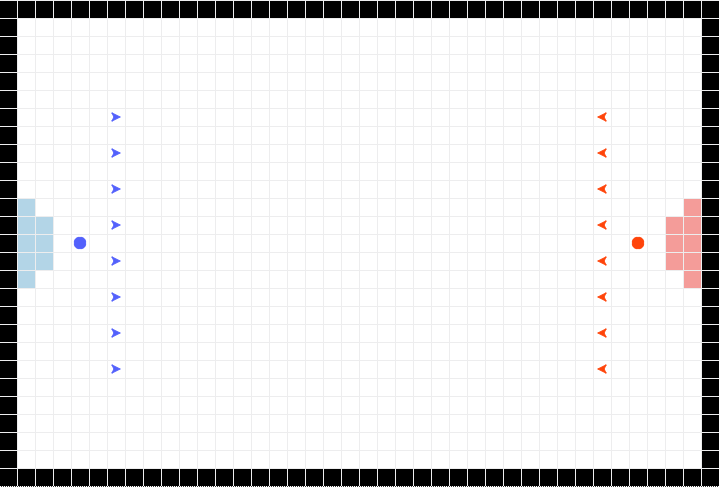
\includegraphics[totalheight=5cm]{figures/flag-ini.png}
	\caption{Configuração inicial do jogo}
	\label{fig:flag-ini}
\end{figure}

Para este jogo foram necessários 5 tipos diferentes de agentes:

\begin{itemize}
	\setlength\itemsep{0pt}
	\item jogador (\textit{player}): possui a capacidade de se mover; capturar e transportar a bandeira do time adversário; e disparar projéteis contra os oponentes.
	\item bandeira (\textit{flag}): é um agente totalmente passivo. Uma vez capturada e entregue pelo time adversário, a bandeira reaparece na posição inicial.
	\item projétil (\textit{fireshot}): é o agente criado quando um jogador realiza um disparo. O projétil movimenta-se em uma trajetória retilínea até atingir algum alvo ou percorrer uma distância máxima. 
	\item zona de entrega (\textit{delivery}): também foi modelada como um agente. Apesar de não poder se mover, a zona de entrega pode ser posicionada em qualquer ponto do \textit{grid}. Sua única ação é recolher a bandeira do time adversário quando algum jogador a trouxer até a sua localização.
	\item barreira (\textit{wall}): assim como na da simulação anterior, a barreira é um agente totalmente inanimado. Sua única função é obstruir o movimento dos jogadores e funcionar como um anteparo para os projéteis.
\end{itemize}

O cenário da simulação representa um campo de batalha discretizado em uma malha de $40 \times 27$ células. Cada time possui sua própria bandeira, oito jogadores e uma área de entrega que ocupa oito células (na prática, existe um agente do tipo \textit{zona de entrega} em cada célula), conforme ilustrado na figura \ref{fig:flag-ini}. A tabela abaixo apresenta a representação gráfica dos agentes:

\begin{table}[h!]
	\begin{center}
		\begin{tabular}{ c  p{8cm} }
			\toprule
			Representação gráfica & Descrição \\ 
			\cmidrule(r){1-1}\cmidrule(lr){2-2}
			
			
\includegraphics[width=5mm, height=5mm]{figures/player.png}
			& 
			Jogador \\
			
			
\includegraphics[width=5mm, height=5mm]{figures/flag.png}
			& 
			Bandeira \\
			
			
\includegraphics[width=5mm, height=5mm]{figures/delivery.png}
			& 
			Zona de entrega \\
			
			
\includegraphics[width=5mm, height=5mm]{figures/fireshot.png}
			& 
			Projétil \\
			
			
\includegraphics[width=5mm, height=5mm]{figures/wall.png}
			& 
			Barreira \\
			
			
\includegraphics[width=5mm, height=5mm]{figures/player_with_flag.png}
			& 
			Jogador transportando a bandeira adversária \\
			
			
\includegraphics[width=5mm, height=5mm]{figures/fired_player_3.png}
			& 
			Jogador atingido por projétil \\
			
			
\includegraphics[width=5mm, height=5mm]{figures/player_stopped.png}
			& 
			Jogador imobilizado \\
			
			
\includegraphics[width=5mm, height=5mm]{figures/fired_wall.png}
			& 
			Colisão do projétil na barreira \\
			\bottomrule
		\end{tabular}
		\caption{Representação gráfica dos agentes e seus estados.}
		\label{tbl:graphics}
	\end{center}
\end{table}

Para manter o equilíbrio do jogo, foram estabelecidas as seguintes regras:

\begin{enumerate}
	\setlength\itemsep{0em}
	\item A posição inicial dos jogadores e das bandeiras é simétrica, de forma a não favorecer nenhuma das duas equipes
	\item A cada passo da simulação cada jogador tem uma probabilidade de 50\% de ser ativado, isto é, de ter a oportunidade de se mover ou fazer um disparo.
	\item Ao ser ativado, o jogador deve escolher se deseja mover-se ou fazer um disparo (não é permitido fazer as duas ações ao mesmo tempo).
	\item Os jogadores podem movimentar-se para qualquer uma das 8 células vizinhas (vizinhança de Moore), desde que elas não estejam ocupadas por algum outro jogador ou por uma barreira.
	\item O jogador tem direito de mudar sua orientação antes de fazer um disparo. Um agente \textit{projétil} será criado na célula em que sua orientação está apontando e irá seguir em linha reta de acordo com esta direção inicial.
	\item O projétil se desloca uma célula por turno e, portanto, tem, em média, o dobro da velocidade de um jogador
	\item O projétil é removido quando atinge um jogador, uma barreira, ou depois de percorrer uma distância máxima de 15 células.	
	\item O jogador que for atingido por um projétil fica imobilizado por 10 turnos.
	\item Após o período de imobilização, o \textit{jogador} atingido fica imune por 5 turnos.
	\item Ao fazer um disparo o jogador fica 3 turnos sem poder disparar novamente (tempo de recarga). No entanto, durante esse período ele continua tendo oportunidade de se mover.
\end{enumerate}

Os \textit{jogadores} são os únicos agentes que utilizam técnicas de inteligência artificial mais elaboradas para a tomada de decisão. Os demais agentes, ou possuem um comportamento puramente determinístico, ou sequer são ativados durante a simulação. 

As \textit{bandeiras}, por exemplo, possuem uma lógica muito simples. Elas são ativadas em todos os turnos e sua única ação é verificar se a sua posição corrente está dentro da zona de entrega da equipe adversária; em caso positivo, ela reaparece na sua posição inicial e incrementa o contador de pontos do time oponente.

Os agentes do tipo \textit{projétil} são criados quando um \textit{jogador} realiza um disparo. Sua posição inicial será a célula vizinha que é apontada pela orientação do jogador que fez o disparo. Essa orientação é repassada para o projétil como um atributo que se mantém constante durante todo o seu ciclo de vida. Assim, a cada novo turno, os projéteis movem-se para a célula vizinha apontada pela orientação definida inicialmente (o que garante um movimento retilíneo). Ao atingir um agente do tipo \textit{jogador}, o projétil altera seu estado para ``imobilizado'' (exceto se ele estiver em condição de imunidade); o que, segundo as regras do jogo, significa que este jogador não poderá ser ativado pelos próximos 10 turnos. Ao colidir com um agente do tipo \textit{jogador} ou \textit{barreira} o projétil modifica sua aparência gráfica (vide tabela \ref{tbl:graphics}) e é então removido no turno seguinte. Finalmente, toda vez que o projétil se movimenta ele incrementa uma de suas variáveis de estado que armazena a distância total percorrida; se esta variável for maior que o alcance máximo do projétil (definido em 15 células) ele é então removido da simulação.

As \textit{zonas de entrega} e as \textit{barreiras}, apesar de terem sido implementadas como agentes para facilitar a modelagem do problema, não possuem nenhum comportamento ativo durante a simulação. Portanto esses agentes sequer foram adicionados ao \textit{scheduler} do modelo. A tabela \ref{tbl:ativacao} resume a como funciona a ativação de cada tipo de agente.

\begin{table}[h!]
	\begin{center}
		\begin{tabular}{ll}
			\toprule
			Agente & Ativação \\ 
			\cmidrule(r){1-1}\cmidrule(lr){2-2}
			Jogador   & Probabilística (50\%) \\
			Bandeiras & Todos os turnos       \\
			Projétil  & Todos os turnos		  \\
			Zona de entrega & Não é ativado (não tem ação) \\
			Barreira        & Não é ativado (não tem ação)\\
			\bottomrule
		\end{tabular}
		\caption{Ativação dos agentes no \textit{scheduler} do modelo.}
		\label{tbl:ativacao}
	\end{center}
\end{table}

Cada equipe possui 8 jogadores que podem assumir uma postura ofensiva (atacante) ou defensiva (defensor). A quantidade de atacantes e defensores da equipe é um parâmetro do modelo que pode ser alterado durante a simulação da partida. Essa configuração define o \textit{esquema tático} do time e o comportamento global de cada jogador. A figura \ref{fig:flag-decision-tree} representa a árvore de decisões executada quando o jogador é ativado; os números em cada nó da árvore foram adicionados para facilitar a identificação dos comportamentos e dos processos de tomada de decisão.

\begin{figure}
	\centering
	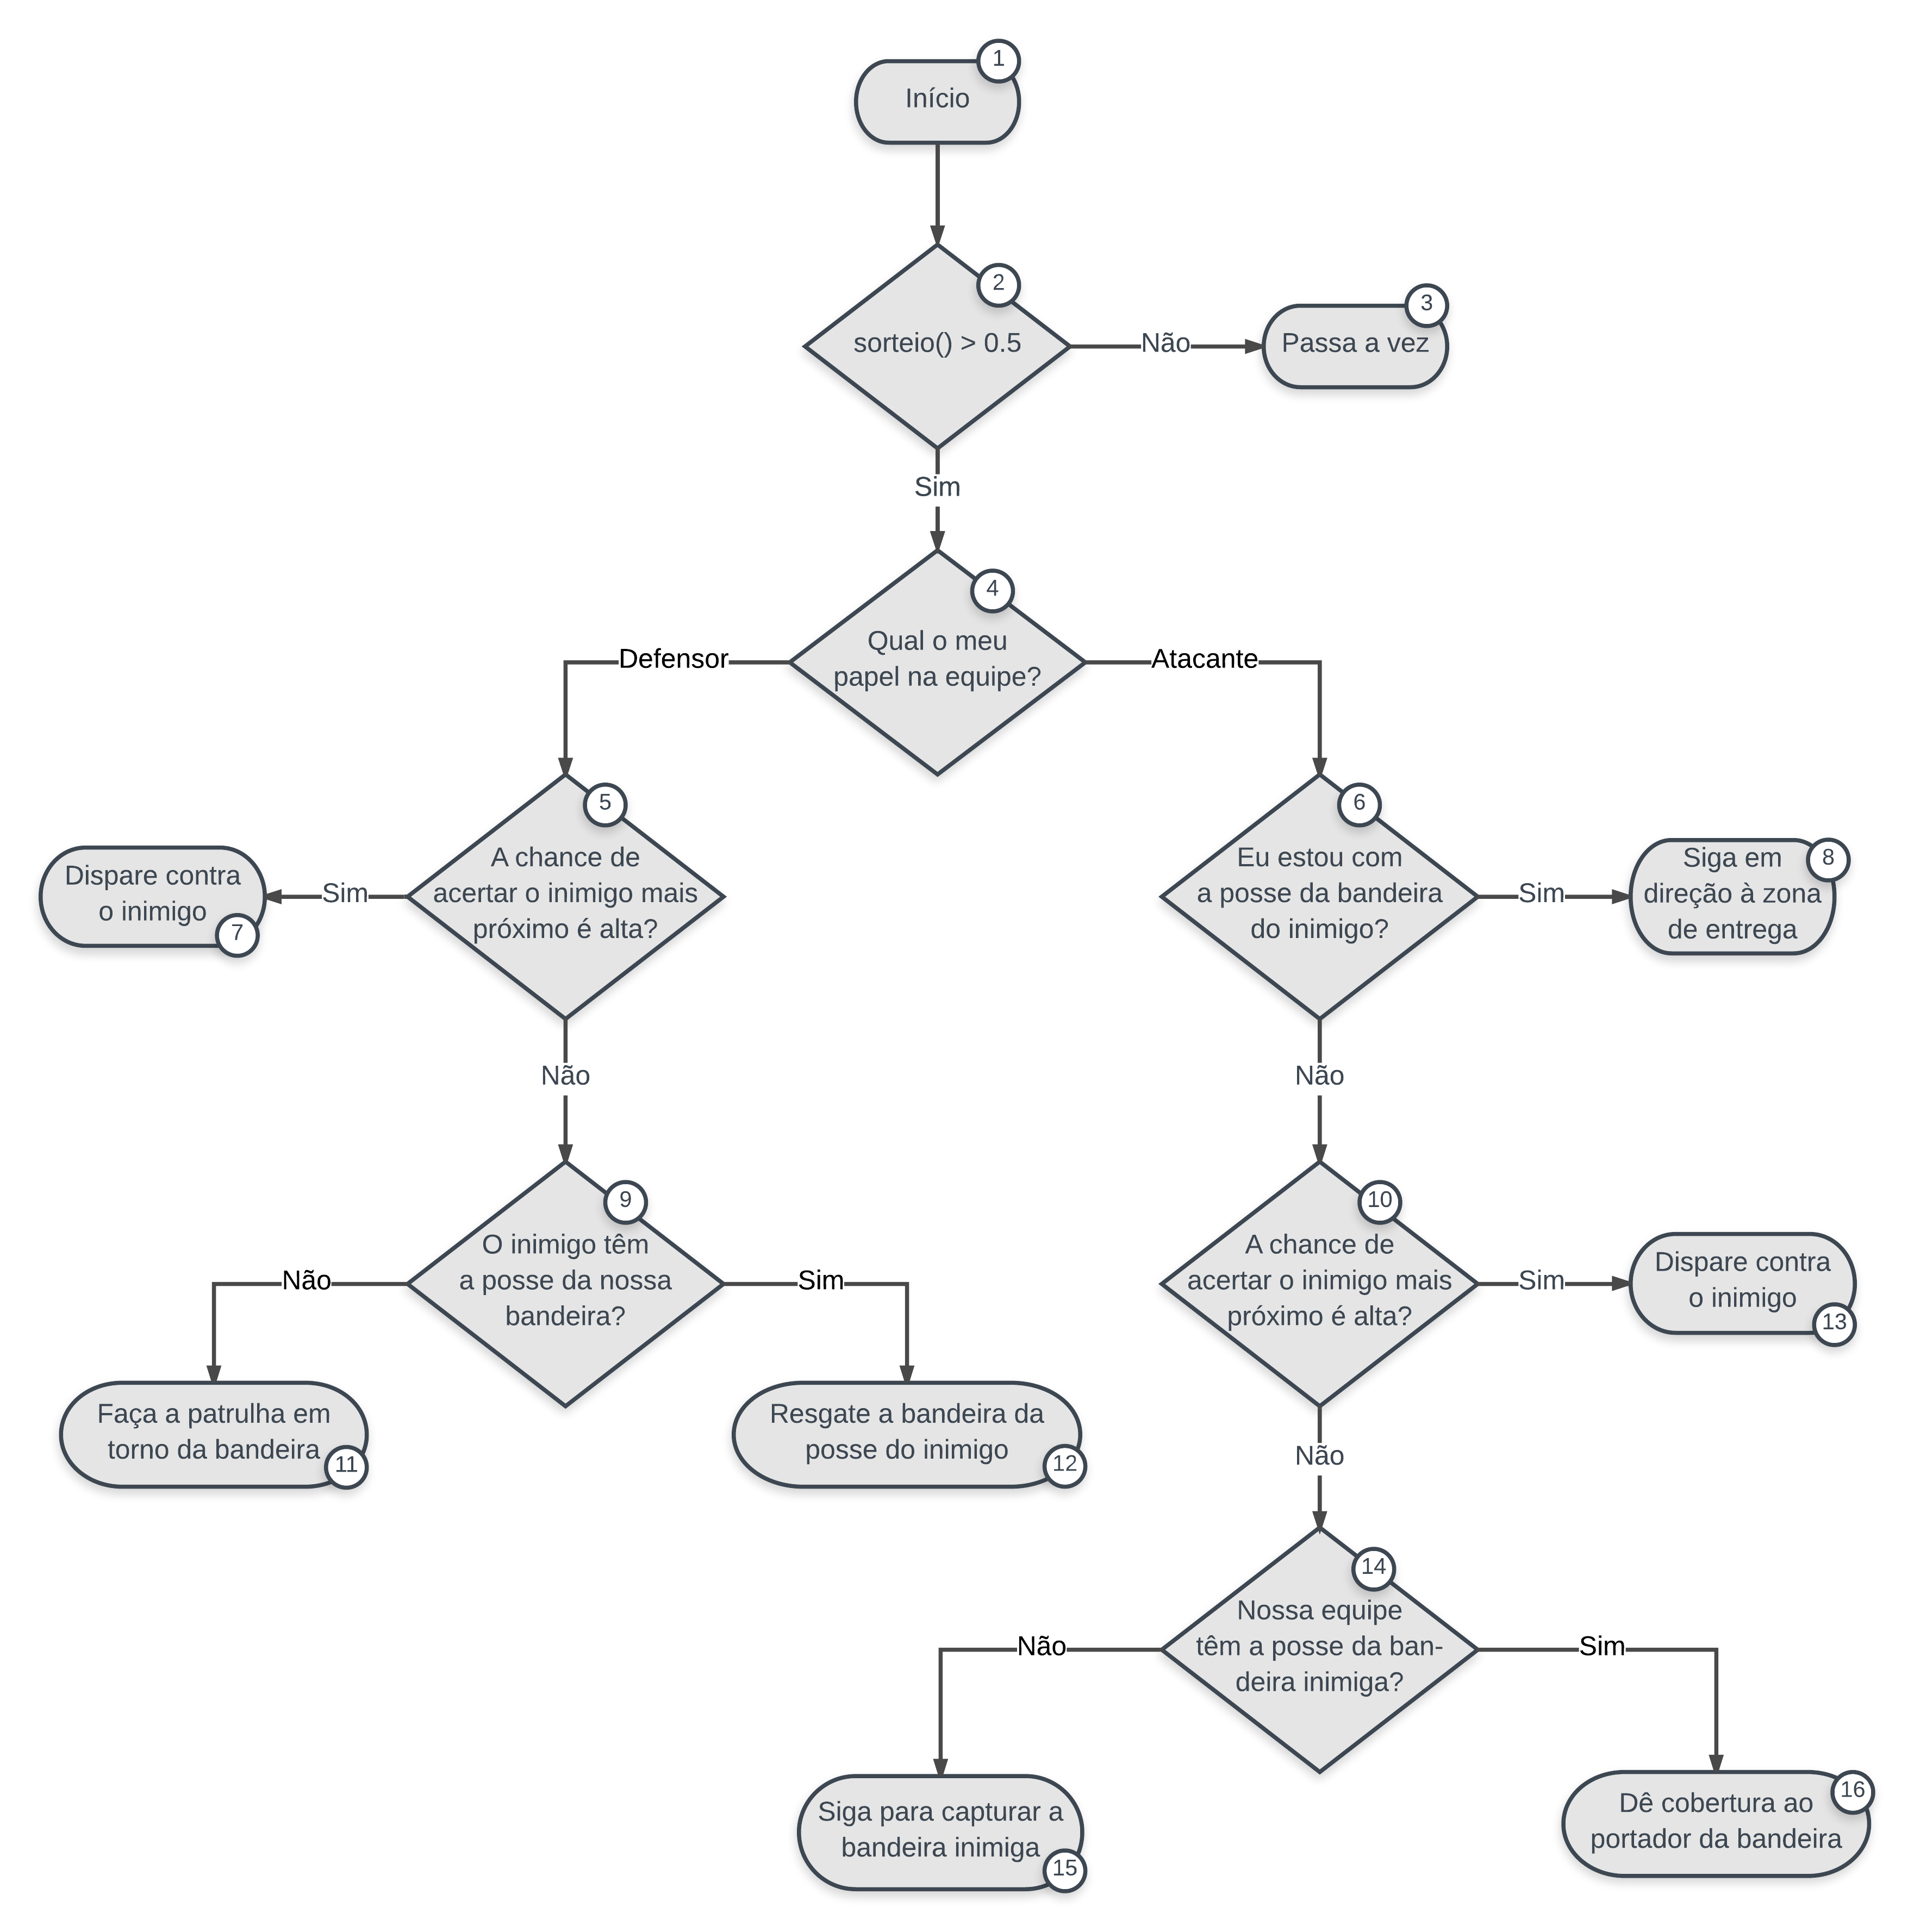
\includegraphics[height=15cm]{figures/flag-tree.png}
	\caption{Árvore de decisão dos \textit{jogadores}.}
	\label{fig:flag-decision-tree}
\end{figure}

Evidentemente, a velocidade dos jogadores deve ser inferior à dos projéteis, caso contrário seria muito improvável acertar um disparo sobre o oponente pois ele poderia esquivar-se com muita facilidade. Além disso, não faz sentido um jogador mover-se na mesma velocidade de um projétil. A condição de ativação definida no nó $2$ da árvore cria uma condição probabilística para a ativação do jogador; isso possui dois efeitos principais: (1) reduz a velocidade dos jogadores, e (2) cada jogador não sabe quando será sua próxima oportunidade de se mover.

A decisão do nó $4$ divide o comportamento dos jogadores de ataque e defesa; esta não é propriamente uma decisão do jogador, mas sim um parâmetro do modelo. Obviamente seria possível fazer com que os jogadores pudessem avaliar a situação do jogo e decidir se devem tomar uma postura ofensiva ou defensiva. Essa decisão poderia ser tomada com base, por exemplo, na distância do jogadores até as bandeiras e na postura dos demais jogadores. No entanto, optamos por manter essa decisão como um parâmetro da simulação; na próxima seção apresentamos o desempenho das equipes em relação ao esquema tático escolhido.

Os jogadores defensivos podem optar por três comportamentos distintos, conforme ilustra a árvore da figura \ref{fig:flag-decision-tree}. Primeiramente, o jogador observa se existe algum jogador inimigo nas proximidades, fato que representa uma ameaça à bandeia ou a sua própria integridade. Então, supondo que a arma do jogador está carregada, ele estima qual é chance de acertar oponente se fizer um disparo; se essa chance superar um determinado limite pré-definido então ele faz o disparo contra o oponente, caso contrário ele segue para o próximo nó de decisão.

Se a chance de sucesso do disparo for baixa, então o jogador defensivo irá observar se o time adversário está com a posse da bandeira de sua equipe. Em caso positivo ele irá seguir e em direção a bandeira para tentar resgatá-la do inimigo, caso contrário, o jogador irá fazer uma patrulha no entorno da bandeira.

Já comportamento dos jogadores de ataque funciona da seguinte maneira: primeiramente, se o jogador já está com a posse da bandeira adversária, então ele deve seguir para a zona de entrega tentando esquivar-se dos inimigos e projéteis. Caso contrário ele, segue a mesma lógica dos jogadores de defesa para verificar se existe algum inimigo próximo que represente uma ameaça e que possa ser atingido por um disparo. Se chance de sucesso do disparo for alta ele lança o projétil, caso contrário ele observa quem está com a posse da bandeira do adversário. Se for alguém da sua própria equipe, ele deve dar cobertura ao portador da bandeira; mas se a bandeira não está na posse da sua equipe ele deve tentar capturá-la.

A árvore de decisão da figura \ref{fig:flag-decision-tree} descreve o comportamento dos jogadores em nível de abstração bastante elevado. Por exemplo ao decidir fazer um disparo, eé necessário verificar se chance de acertar o adversário é suficientemente alta. Para isso é necessário saber em qual direção atirar e como calcular a chance de sucesso. Esta decisão foi implementada usando o conceito de \textit{mapas de influência} (ver \cite{millington2016artificial}). Cada jogador possui seu próprio de campo de influência, que modifica o mapa de influência do ambiente; da mesma forma os projéteis também possuem um campo de influência dentro do ambiente. A decisão de fazer o disparo é implementada através da soma do produto ponto-a-ponto do campo de influência do projétil a ser criado sobre o mapa de influência dos jogadores (jogadores aliados têm uma influência negativa e jogadores inimigos têm influência positiva). Se este somatório for alto significa que o campo de influência do projétil cruza com o campo de influência dos jogadores adversários, e, portanto, o disparo tem uma chance razoável de acertar o alvo. Por outro lado, valores negativos indicam que o disparo pode acertar jogadores aliados.

O campo de influência dos jogadores e dos projéteis, assim como o valor limiar para decidir efetuar o disparo, foram definidos após alguns testes empíricos. Os campos de influência dos projéteis e jogadores podem ser consultados no arquivo \textit{/projects/flag/influence\_masks.py} do repositório deste projeto.

Além dos mapas de influência, utilizamos também o algoritmo $A^*$ para traçar a rota dos jogadores ao tentar capturar e entregar a bandeira do adversário. O custo dos movimentos no algoritmo $A^*$ também leva em consideração os mapas de influencia dos jogadores e projéteis, para evitar rotas que: (1) cruzem com o trajeto de um projétil (evita o risco de ser atingido), (2) passem muito próximo de um inimigo -evita que o inimigo faça um disparo \textit{à queima roupa}), ou (3) passem muito próximo de outro jogador aliado (evita ataques concentrados, o que, em geral, tende a ser uma estratégia ruim).

\section{Resultados}
\label{sec:resultados}

Nesta seção apresentamos alguns resultados interessantes sobre os modelos apresentados neste trabalho.

\subsection{Regiões da estação com maior circulação de pessoas}
\label{subsec:metro_heatmap}

Em uma situação real, pode ser interessante identificar quais são as regiões da estação que apresentam a maior circulação de pessoas, por exemplo, para evitar que essas áreas sejam obstruídas ou ainda para posicionar e precificar anúncios publicitários.

A figura \ref{fig:heatmap} representa um mapa de calor da estação, indicando as regiões com mair circulação de passageiros. Cada cor indica pessoas caminhando em um determinado sentido, tons mais escuros representam as regiões com maior circulação de passageiros.

\begin{figure}[H]
	\centering
	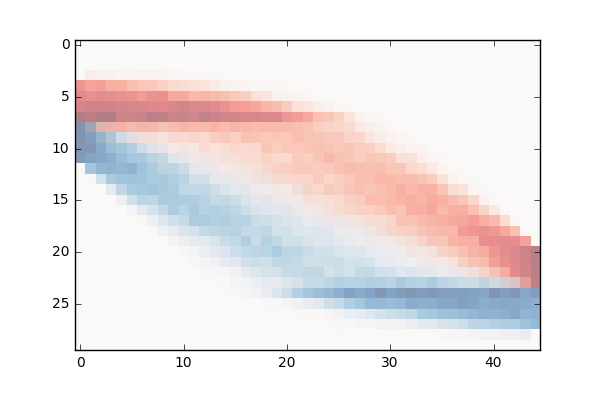
\includegraphics[totalheight=7cm]{figures/heatmap.png}
	\caption{Mapa de calor das regiões com maior circulação de passageiros.}
	\label{fig:heatmap}
\end{figure}

Observando a figura \ref{fig:heatmap}, é possível verificar que as pessoas começam a se dispersar após cruzarem a roleta de entrada e voltam a convergir ao se aproximarem das roletas de saída. Este é um comportamento bastante elementar, mas que não foi explicitamente programado na construção do modelo.

\subsection{Tempo e distância percorrida para atravessar a estação}
\label{subsec:tempo_travessia}

Outra característica importante para ser analisada no modelo de fluxo de passageiros é o tempo médio que as pessoas levam para atravessar a estação. Intuitivamente, podemos supor que quanto maior a circulação de pessoas na estação, a movimentação fica mais restrita e, portanto, maior deve ser o tempo de travessia.

Como os agentes possuem velocidades muito diferentes uns dos outros, o tempo médio de travessia pode ter uma variação muito grande. Portanto, ao invés de contabilizar o tempo total que o agente levou para atravessar a estação, optamos por medir: (1) a distância total percorrida pelo agente, e (2) o número de vezes que o agente foi ativado. O primeiro indicador considera a distância euclidiana entre duas células vizinhas, penalizando os trajetos tortuosos; já a segunda medida, penaliza os casos em que o agente teve a oportunidade de se mover, mas dada as circunstâncias, preferiu continuar na mesma posição.

As figuras \ref{fig:dists_boxplot} e \ref{fig:atvs_boxplot} demonstram como variam a distância percorrida pelos agentes e o número de vezes que eles são ativados em função do fluxo de pessoas nos acessos de entrada e saída. Estes gráficos foram gerados, mantendo o fluxo de passageiros constante por $1000$ passos de tempo para cada simulação. Para facilitar a visualização limitamos o intervalo das ordenadas nas duas figuras, o que ocultou alguns \textit{outliers} mais extremos.

\begin{figure}[H]
	\centering
	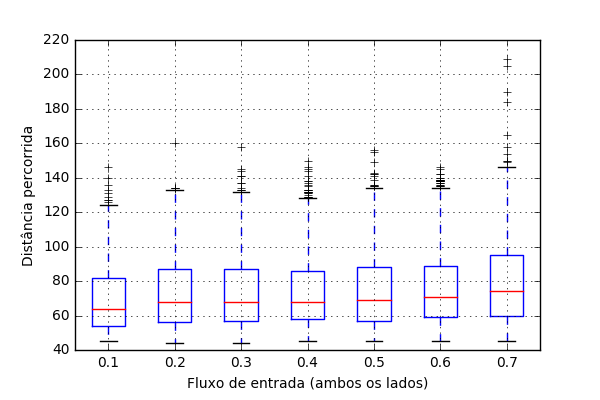
\includegraphics[totalheight=7cm]{figures/dist_boxplot.png}
	\caption{Distância percorrida em função do fluxo de passageiros.}
	\label{fig:dists_boxplot}
\end{figure}

\begin{figure}[H]
	\centering
	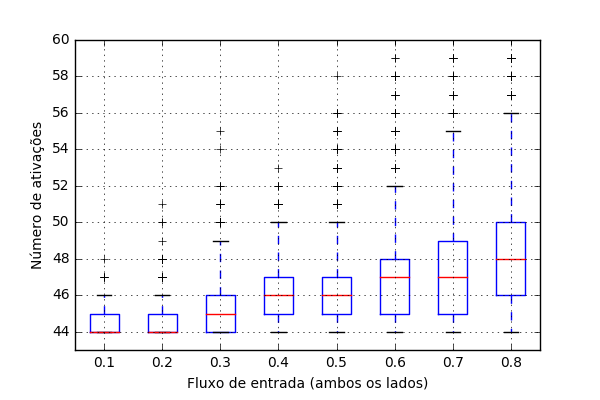
\includegraphics[totalheight=7cm]{figures/ativs_boxplot.png}
	\caption{Número de ativações em função do fluxo de passageiros.}
	\label{fig:atvs_boxplot}
\end{figure}

Conforme o esperado, os gráficos das figuras \ref{fig:dists_boxplot} e \ref{fig:atvs_boxplot} confirmam que tanto a distância percorrida, quanto o tempo de travessia aumentam à medida que fluxo de passageiros cresce. Um fato interessante é que o aumento das medianas é relativamente lento, mas a variância da distribuição cresce bastante à medida que o fluxo de passageiros aumenta.

\subsection{Esquema tático das equipes}
\label{subsec:esquema_tatico}

O esquema tático de cada equipe, isto é, a proporção entre número de atacantes e defensores do time são parâmetros da simulação. A tabela \ref{tbl:flag_scoreboard} apresenta o resultado de uma partida de $5000$ passos de tempo para todas combinações possíveis de esquemas táticos entre as duas equipes.

A primeira linha indica o esquema tático da equipe vermelha, enquanto que a primeira coluna indica o esquema tático da equipe azul. Utilizamos cores distintas para facilitar a visualização. A notação \blu{3A$\times$5D} indica que time azul joga com 3 atacantes (\blu{$3A$}) e 5 defensores (\blu{$5D$}) As células representam a pontuação de cada equipe ao final da partida. 

\begin{table}[H]
	\begin{center}
		\begin{tabular}{cccccccc}
			\toprule
			Esquema tático & \red{1A$\times$7D}  & \red{2A$\times$6D}  & \red{3A$\times$5D}  & \red{4A$\times$4D}  & \red{5A$\times$3D}  & \red{6A$\times$2D}  & \red{7A$\times$1D}\\
			\cmidrule(r){1-8}
			\blu{1A$\times$7D}    & \score{10}{10} & \score{11}{18} & \score{09}{26} & \score{11}{27} & \score{15}{25} & \score{15}{29} & \score{09}{15} \\
			\blu{2A$\times$6D}    & \score{17}{11} & \score{16}{20} & \score{17}{22} & \score{20}{25} & \score{22}{26} & \score{24}{32} & \score{24}{30} \\
			\blu{3A$\times$5D}    & \score{18}{12} & \score{21}{17} & \score{22}{24} & \score{22}{29} & \score{24}{28} & \score{29}{31} & \score{32}{37} \\
			\blu{4A$\times$4D}    & \score{22}{13} & \score{24}{20} & \score{23}{22} & \score{26}{29} & \score{30}{34} & \score{28}{32} & \score{32}{35} \\
			\blu{5A$\times$3D}    & \score{24}{15} & \score{20}{22} & \score{27}{30} & \score{28}{30} & \score{29}{32} & \score{34}{36} & \score{34}{35} \\
			\blu{6A$\times$2D}    & \score{25}{19} & \score{26}{23} & \score{31}{30} & \score{31}{33} & \score{31}{35} & \score{33}{36} & \score{37}{37} \\
			\blu{7A$\times$1D}    & \score{13}{13} & \score{27}{28} & \score{29}{30} & \score{33}{35} & \score{35}{38} & \score{33}{39} & \score{35}{37} \\

			\bottomrule
		\end{tabular}
		\caption{Representação gráfica dos agentes e seus estados.}
		\label{tbl:flag_scoreboard}
	\end{center}
\end{table}

Naturalmente podemos observar que as pontuações das equipes é relativamente baixa quando ambas adotam um esquema tático muito defensivo. Compare, por exemplo, a média das pontuações das equipes nas submatrizes $3\times3$ no canto superior esquerdo (esquemas táticos defensivos) e no canto inferior direito (esquemas táticos ofensivos).

De modo geral, os pontos marcados por uma equipe tende a aumentar quando colocamos mais atacantes. No entanto, uma exceção interessante acontece quando uma equipe está com 7 atacantes e a outra com 7 defensores; nos dois casos simulados, a pontuação marcada pela equipe com 7 atacantes foi bem inferior ao esquema tático com 6 atacantes. Durante a simulação percebemos que isso ocorre pois o número de jogadores (aliados e adversários) cercando a bandeira é muito grande, obstruindo o caminho do jogador que está transportando a bandeira.

Conforme discutimos na seção \ref{sec:agentes} a modelagem baseada em agentes é essencialmente estocástica. Portanto, para obter resultados significativos é importante realizar várias simulações e observar o comportamento médio global do sistema à medida que os parâmetros são modificados. No nosso caso, haviam duas possibilidades de tentar neutralizar o efeito aleatório das simulações: (1) simular um número muito grande de partidas, ou (2) simular uma partida por um tempo muito prolongado. Obviamente, o ideal é combinar as duas abordagens para neutralizar ao máximo as influências aleatórias, entretanto, por restrições de tempo e custo computacional, optamos por seguir a segunda abordagem.

\section{Conclusão}
\label{sec:conclusao}

Neste trabalho apresentamos como o conceito de modelagem baseada em agentes pode ser aplicado no contexto de jogos de computador. O comportamento dos agentes foi modelado utilizando-se técnicas de inteligência artificial comumente empregadas em na construção de jogos: árvores de decisão, mapas de influência, função de avaliação estática, e o algoritmo \textit{A*}.

Para ilustrar a utilização desses conceitos, apresentamos dois modelos distintos: a simulação do fluxo de passageiros em uma estação de metrô e o jogo de competição pela bandeira adversária. 

O primeiro caso envolve um modelo bastante simples em que os passageiros se comportam de forma puramente egoísta. A tomada de decisão dos passageiros resume-se à minimizar uma função de avaliação que considera apenas o custo do movimento e a distância até a saída mais próxima. Apesar da simplicidade do modelo, os resultados em escala macro levaram à um comportamento bastante verissímil; o suficiente, por exemplo, para produzir uma animação para um filme ou jogo de computador.

Por outro lado, o modelo de competição pela bandeira exige que os agentes se comportem seguindo uma estratégia bem mais elaborada. Os jogadores da mesma equipe precisam atuar de forma colaborativa entre si e competitiva com os times da outra equipe. Estes objetivos produzem uma diversidade de comportamentos, que inclui ações como: (1) guardar sua própria bandeira, (2) resgatar sua bandeira da posse do adversário, (3) atacar a bandeira adversária, (4) carregar a bandeira do adversário até a área de entrega, ou (5) dar cobertura ao jogador que está carregando a bandeira. 

Uma vez que o jogador decide qual comportamento ele deve tomar, é necessário decidir também para qual direção ele deve se mover (ou em qual direção deve disparar), de forma a atingir os objetivos pretendidos com o comportamento escolhido. Essas decisões são feitas com base em uma análise sobre o estado atual do ambiente e dos agentes, tanto aliados como adversários, o que torna o processo de decisão bastante complexo.

No entanto, ainda é possível aprimorar os modelos propostos em vários aspectos. Algumas propostas de trabalhos futuros incluem: (1) associar grandezas físicas usando dados realistas ao modelo de fluxo de passageiros, considerando, por exemplo, a área média ocupada por uma pessoa, as dimensões da estação, e a velocidade das pessoas; (2) rever as regras gerais do jogo de capturar a bandeira, de tal forma que o resultado das equipes fique mais sensível à escolha de um esquema tático e da estratégia de jogo dos agentes; (3) implementar uma lógica para que o jogador possa alternar entre atacante e defensor dependendo de sua posição e da situação do jogo; (4) implementar comportamentos mais elaborados para os jogadores, levando em consideração previsões sobre as ações mais prováveis do adversário.

\section*{Referências}

\bibliography{references.bib}
\bibliographystyle{unsrtnat}

\end{document}
